\subsection{Muon system}
\label{sec:muon}

The purpose of the muon system in the CMS experiment is to identify and reconstruct the trajectories of muons.
These reconstructed trajectories are used both for triggering (Section \ref{sec:trigger}) and 
for offline analyssis.
Three types of gaseous detectors are used to measure muons in the CMS detector.
Since muons are minimum ionizing particles (MIPs) 
\nomenclature{MIP}{Minimum ionizing particle}
and do not generally interact with the inner regions of the 
detector, muon systems are typically placed outside of the tracking and calorimetry systems
in most particle detectors.
In the case of CMS, the muon system rests outside of the solenoid and covers the pseudorapidity 
region $|\eta| < 2.4$.
A plot showing the number of interaction lengths as a function of pseudorapidity 
is given in Figure \ref{fig:muon-interaction-lengths}.
\begin{figure}
  \centering
    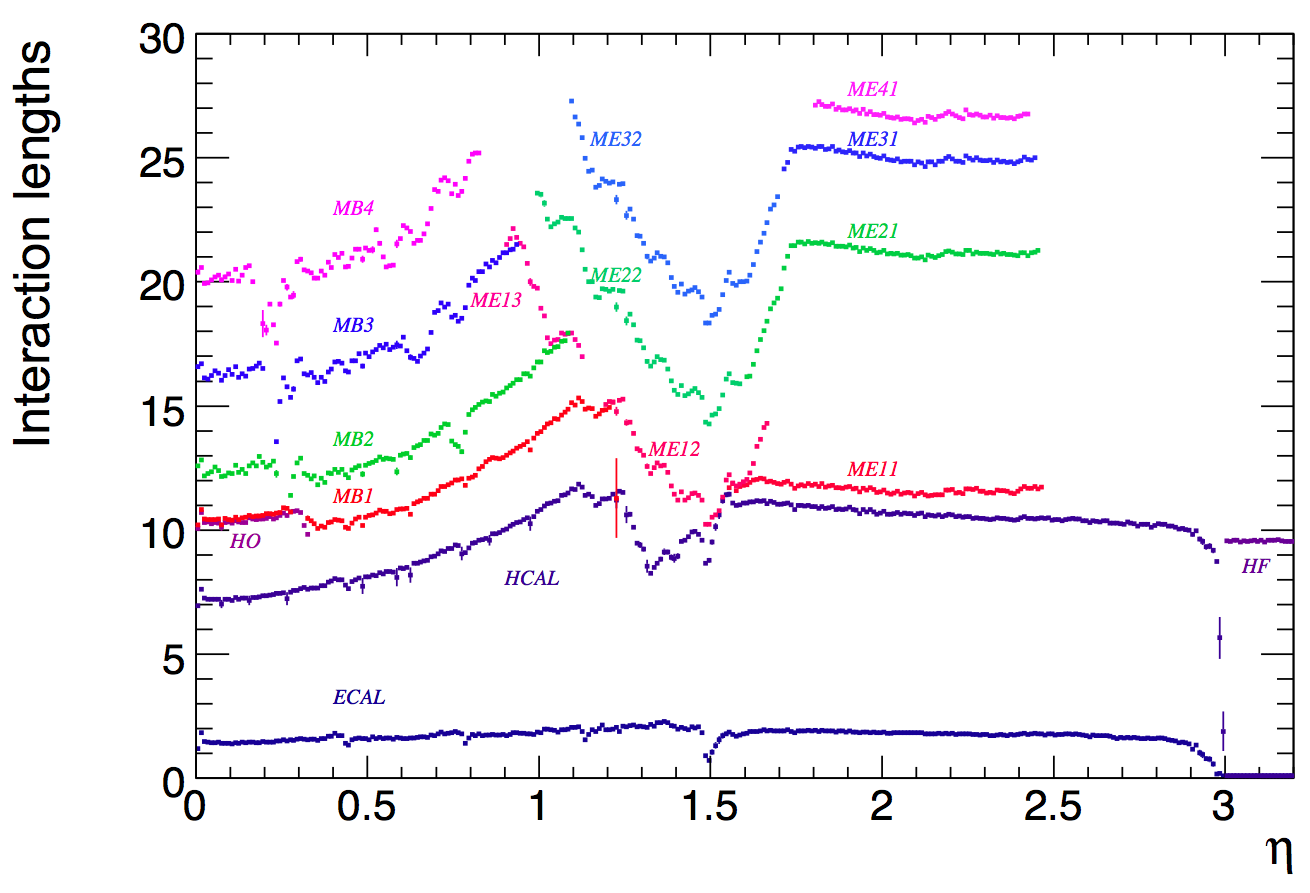
\includegraphics[width=0.8\textwidth]{tex/cms/fig/muon-interaction-lengths.png}
  \caption{Material thickness of the CMS detector in interaction legnths as a function of pseudorapidity.
    All muon barrel and endcap stations are labeled \cite{cms-jinst}.}
  \label{fig:muon-interaction-lengths}.
\end{figure}
This region includes a wide range of incident muon rates,
neutron-induced background rates, and magnetic field strengths.  The choice 
of which detector technologies to use is strongly dependent on these conditions.
In the barrel ($|\eta| < 1.2)$, where the incident muon rate, the neutron-induced background rate, and
the residual magnetic field are relatively low, drift tube chambers (DTs)
\nomenclature{DT}{Drift tube chambers}
with rectangular drift cells are used.
In the endcaps, where the incident muon rate, the neutron induced background rate,
and the residual magnetic field are relatively high, cathode strip chambers (CSCs)
\nomenclature{CSC}{Cathode strip chambers}
are used.
In addition, resistive plate chambers (RPCs)
\nomenclature{RPC}{Resistive plate chambers}
are used in both the barrel and the endcap ($|\eta| < 1.6$).  RPCs have a faster response and a 
better time response than the DTs and CSCs, but they have a coarser position resolution.
This allows them to unambiguously identify the bunch crossing associated with a reconstructed muon.
In total, the muon system is made up of 25,000 $\text{m}^2$ of active detection area and nearly
1 million electronic channels.
The layout of the CMS muon system is shown in a schematic in Figure \ref{fig:muon}.

\begin{figure}
  \centering
  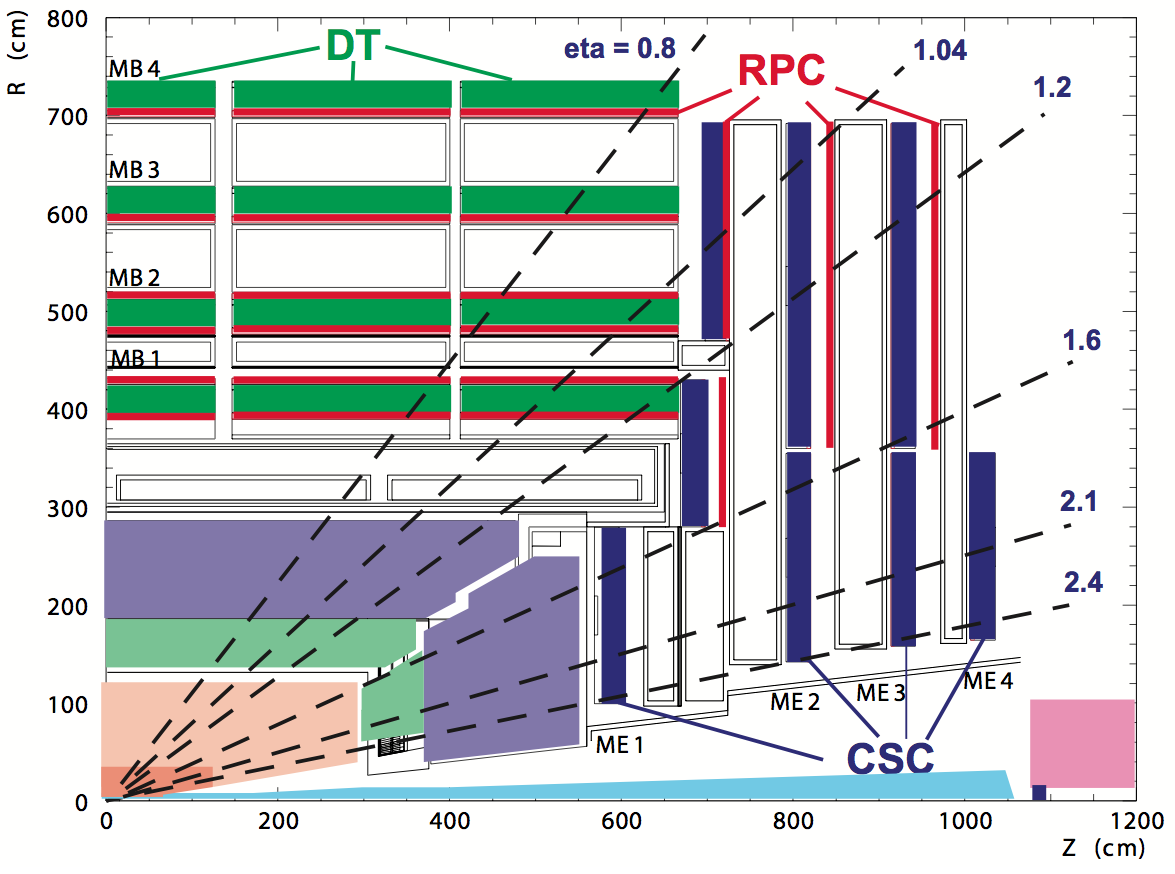
\includegraphics[width=1.0\textwidth]{tex/cms/fig/muon-schematic.png}
  \caption{A schematic cross section of the CMS muon system.  Only one quarter of the entire
    muon system is represented. The numbering scheme for the various stations (MB1-4 in the barrel,
    ME1-4 in the endcap) is clearly labeled.
    The three subsystems: the drift tube chambers (DTs), 
    resistive plate chambers (RPCs), and cathode strip chambers (CSCs) are also shown
    \cite{cms-tdr}.}
  \label{fig:muon}
\end{figure}

The muon system in the barrel region is organized into four layers or ``stations''
which are separated by layers of the iron return yoke.
These layers are located at radii of approximately 4.0, 4.9, 5.9, and 7.0m from the IP.
The stations are labeled MB1-4, with MB1 located closest to the IP.  The stations are further
divided into five ``wheels'', which are labeled from YB-2 (farthest in the $z$-minus direction)
to YB+2 (farthest in the $z$-plus direction), following the segmentation of the iron
return yoke.  Each of these 5 wheels is split in $\phi$ into 12 sectors, and each sector 
covers $30^{\circ}$ of azimuthal angle.  Sectors in different stations are staggered so that
a high-\pt muon near a sector boundary would interact with at least 3 of the 4 stations.
Stations MB1 and MB2 are made up of packages consisting of one DT chamber placed between
two RPCs.  Stations MB3 and MB4 are made up of packages consisting of one DT chamber placed with
a layer of 1, 2, or 4 RPCs.  Stations MB1, MB2, and MB3 provide measurements on muon
coordinates in the $r-\phi$ plane and on the $z-$axis, while  MB4 only provides measurements in the $r-\phi$ plane.
These measurements allow a muon track to be reconstructed with a $\phi$ positional precision better than 100~$\mu\text{m}$
and a directional precision better than 1 mrad.

The muon system in the endcap region is arranged into 4 stations for each of the 2 endcaps.
These stations are labeled ME1-4, where ME1 is the closest to the IP.  The stations 
are each divided into three rings, labeled 1-3, where ring 1 is closest to the beamline.
Each individual CSC is trapezoidal in shape and contains 6 gas gaps.  Each gap
contains radial cathode strips and a set of anode wires that run perpendicularly to the
strips.  As in the barrel, the CSCs are overlapped to avoid gaps of uninstrumented areas.
There are 36 CSCs in each ring of the muon endcap system, except for the innermost ring
in stations ME2, ME3, and ME4, where there are 18 CSCs.  
In addition, only the innermost ring of ME4 has been installed, and 5 spare CSCs were installed
on the outermost ring of ME4 on the $z-$plus side.  There are a total of 468 CSCs in all of CMS, excluding the extras in ME4/2.
Each CSC measures up to 6 spatial
coordinates ($r$, $\phi$, $z$), one for each of its layers.
36 RPCs in total are mounted only in the 2 outer rings of each of the endcap stations.
The endcap muon system allows a muon track to be reconstructed with a $\phi$ positional precision of around 200~$\mu\text{m}$
and a directional precision of about 10 mrad \cite{cms-tdr,cms-jinst}.
